%% AMS-LaTeX Created with the Wolfram Language for Students - Personal Use Only : www.wolfram.com

\documentclass{article}
\usepackage{amsmath, amssymb, graphics, setspace}

\newcommand{\mathsym}[1]{{}}
\newcommand{\unicode}[1]{{}}

\newcounter{mathematicapage}
\begin{document}

\begin{doublespace}
\noindent\(\pmb{\text{Show}[\text{Plot}[\{x{}^{\wedge}2,-x{}^{\wedge}2\}, \{x, -0.1, 0.1\}, \text{PlotStyle} \to  \{\{\text{Blue}, \text{Dashed},
\text{Opacity} [0.3]\}\}],}\\
\pmb{\text{Plot}[x{}^{\wedge}2\text{Sin}[1/x], \{x, -0.1, 0.1\}]]}\)
\end{doublespace}

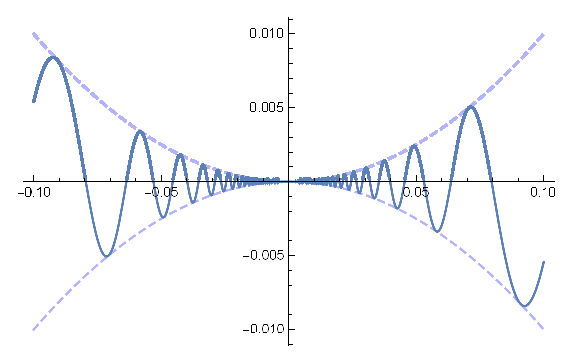
\includegraphics{plots_gr1.eps}

\begin{doublespace}
\noindent\(\pmb{\text{Show}[\text{Plot}[\{x{}^{\wedge}2 + x/2,-x{}^{\wedge}2 + x/2\}, \{x, -0.1, 0.1\}, }\\
\pmb{\text{PlotStyle} \to  \{\{\text{Blue}, \text{Dashed}, \text{Opacity} [0.3]\}\}],}\\
\pmb{\text{Plot}[x/2 + x{}^{\wedge}2\text{Sin}[1/x], \{x, -0.1, 0.1\}]]}\)
\end{doublespace}

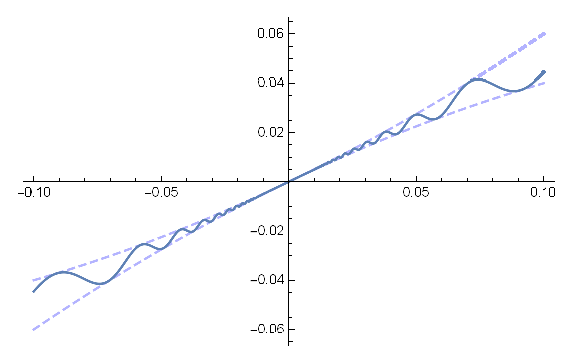
\includegraphics{plots_gr2.eps}

\begin{doublespace}
\noindent\(\pmb{\text{Plot}[\{1/x, -x + 1/2\}, \{x, -5, 5\}]}\)
\end{doublespace}

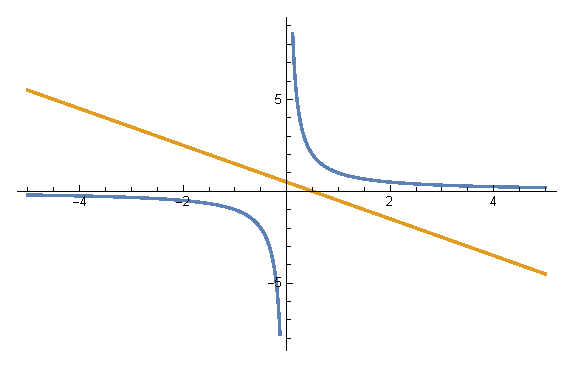
\includegraphics{plots_gr3.eps}

\end{document}
